\documentclass{article}
\usepackage[utf8]{inputenc}
\usepackage[T1]{fontenc}
\usepackage{graphicx}
\usepackage{hyperref}
\usepackage{geometry}
\geometry{margin=1in}

\title{BYRHUS}
\date{Encyclopaedia Britannica (1771)}

\begin{document}
\maketitle

\section*{Historical source}
\textbf{Entry ID:} \texttt{entry-byrhus-2250} \\
\textbf{Volume ID:} 144133901 \\
\textbf{Character Count:} 328

\subsection*{Extracted Text}
BYRHUS, in zodogy, an order of infects belonging to the order of coloroptera. The feelers are clavated, pretty folkl, and a little compelled. These are five species, all of which are to be found on particular plants and principally disfiguplified from each other by the colour and figure of the clytra or cruttaccous wing cases.



\section*{Source record}
\begin{itemize}
\item \textbf{Dataset:} \texttt{NationalLibraryOfScotland/encyclopaedia\_britannica\_illustrated}
\item \textbf{Dataset Revision:} \texttt{309f765b1ecc83e0a7f7762e44b4a927a7555443}
\item \textbf{Page ID:} \texttt{britannica:309f765b1ecc83e0a7f7762e44b4a927a7555443:train:2250} \\
  \textbf{Filename:} \texttt{page-2250-75315f455009.jpg} \\
  \textbf{Row Index:} 2250 \\
  \textbf{SHA256:} \texttt{75315f45500988da...}
\end{itemize}

\begin{figure}[h]
\centering
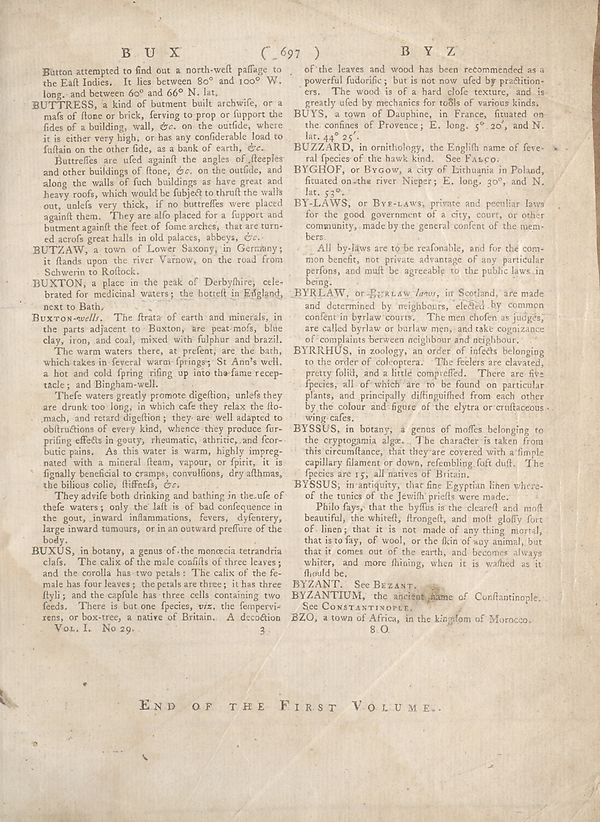
\includegraphics[width=0.85\textwidth]{../scans/page-2250-75315f455009.jpg}
\caption*{Source scan: \texttt{page-2250-75315f455009.jpg}}
\end{figure}

\end{document}
